% Presentacion de avance: benchmark VQC/VQN (pure-v1)
% Compilar desde esta carpeta: pdflatex avances_vqc.tex (dos veces)
% Las figuras se leen de vqc_scorecard/figures/, no se copian.
\documentclass[aspectratio=169,10pt]{beamer}
\usepackage[utf8]{inputenc}
\usepackage[T1]{fontenc}
\usepackage{courier}
\usepackage{helvet}
\usepackage{booktabs}
\usepackage{tabularx}
\usepackage{graphicx}
\usepackage{xcolor}
\usepackage[most]{tcolorbox}
\graphicspath{{../../figures/}}

\usetheme{default}
\setbeamertemplate{navigation symbols}{}
\setbeamertemplate{footline}{\hfill\scriptsize\insertframenumber\,/\,\inserttotalframenumber\hspace{1em}\vspace{0.6em}}
\setbeamerfont{frametitle}{series=\bfseries,size=\large}
\setbeamercolor{frametitle}{fg=black}
\setbeamercolor{title}{fg=black}
\setbeamertemplate{itemize item}{\textbullet}

\definecolor{azul}{HTML}{1F4E9A}
\definecolor{verde}{HTML}{2E7D32}
\definecolor{ambar}{HTML}{B7860B}
\newtcolorbox{azulbox}[1]{enhanced,colback=azul!5,colframe=azul,boxrule=0.6pt,arc=0pt,left=4pt,right=4pt,top=2pt,bottom=3pt,fonttitle=\bfseries\small,coltitle=azul,colbacktitle=azul!5,attach title to upper={\par\smallskip},title={#1}}
\newtcolorbox{verdebox}[1]{enhanced,colback=verde!6,colframe=verde,boxrule=0.6pt,arc=0pt,left=4pt,right=4pt,top=2pt,bottom=3pt,fonttitle=\bfseries\small,coltitle=verde,colbacktitle=verde!6,attach title to upper={\par\smallskip},title={#1}}
\newtcolorbox{ambarbox}[1]{enhanced,colback=yellow!7,colframe=ambar,boxrule=0.6pt,arc=0pt,left=4pt,right=4pt,top=2pt,bottom=3pt,fonttitle=\bfseries\small,coltitle=ambar!80!black,colbacktitle=yellow!7,attach title to upper={\par\smallskip},title={#1}}

\newcommand{\ok}{\textcolor{verde}{\textbf{Completo}}}
\newcommand{\pend}{\textcolor{ambar!80!black}{\textbf{Pendiente}}}
\newcommand{\inc}{\textcolor{ambar!80!black}{\textbf{Parcial}}}

\title{Benchmark reproducible de circuitos cuánticos variacionales (VQC/VQN) para NLP bajo restricciones NISQ}
\author{Luis Daniel González Alcocer}
\date{30 de octubre de 2026}

\begin{document}

% ---------------------------------------------------------------- 1
\begin{frame}
\vfill
\begin{tcolorbox}[colback=azul!12,colframe=azul!12,arc=4pt,halign=center,top=10pt,bottom=10pt]
{\Large\bfseries Benchmark reproducible de circuitos\\ cuánticos variacionales (VQC/VQN)\\ para NLP bajo restricciones NISQ}
\end{tcolorbox}
\vspace{1.5em}
\centering Luis Daniel González Alcocer\\[0.3em] Tecnológico de Monterrey\\[0.3em] 30 de octubre de 2026
\vfill
\end{frame}

% ---------------------------------------------------------------- 2
\begin{frame}{2. Agenda}
\begin{columns}[T]
\column{0.48\textwidth}
\begin{enumerate}\setcounter{enumi}{2}
\item Contexto y pregunta de investigación
\item Diseño experimental
\item Arquitecturas evaluadas
\item Descriptores del circuito
\item Resultados: descriptores
\end{enumerate}
\column{0.48\textwidth}
\begin{enumerate}\setcounter{enumi}{7}
\item Resultados: tarea IMDb y CoLA
\item Resultados: ruido
\item Hipótesis pre-registradas
\item Repositorio y reproducibilidad
\item Pendientes y conclusiones
\end{enumerate}
\end{columns}
\end{frame}

% ---------------------------------------------------------------- 3
\begin{frame}{3. Contexto y pregunta de investigación}
\begin{azulbox}{Pregunta central}
Qué propiedades de un circuito cuántico variacional (número de qubits, profundidad, codificación y estructura del ansatz) explican su desempeño, su entrenabilidad y su robustez al ruido cuando el circuito es el único componente que aprende.
\end{azulbox}
\begin{columns}[T]
\column{0.48\textwidth}
\begin{verdebox}{Lo que este proyecto no es}
No busca demostrar ventaja cuántica. Los modelos clásicos se reportan como referencia, no como competidores.
\end{verdebox}
\column{0.48\textwidth}
\begin{ambarbox}{Lo que este proyecto es}
Un benchmark reproducible de siete familias VQC publicadas, con hipótesis escritas antes de correr los experimentos.
\end{ambarbox}
\end{columns}
\end{frame}

% ---------------------------------------------------------------- 4
\begin{frame}{4. Diseño experimental}
\small
\begin{tabularx}{\textwidth}{@{}lXl@{}}
\toprule
\textbf{Fase} & \textbf{Pregunta que responde} & \textbf{Estado}\\
\midrule
Descriptores & Qué tan expresivo, entrelazado y entrenable es cada circuito antes de entrenarlo (P1 a P6, G1 a G6). & \ok\\
fair-v1 & Protocolo híbrido con capas clásicas grandes. Archivado: las capas clásicas hacían el trabajo. & \ok\\
pure-v1 IMDb & Desempeño cuando solo el circuito aprende. 7 familias, $n\in\{4,6,8\}$, $d\in\{1,3,5\}$, 10 semillas. & \ok\\
pure-v1 CoLA & Mismo protocolo en aceptabilidad gramatical. & \inc\ ($n=4$)\\
Ruido & Cómo cambia la predicción con ruido de hardware ($n=4$). & \ok\\
\bottomrule
\end{tabularx}
\end{frame}

% ---------------------------------------------------------------- 5
\begin{frame}{4. Diseño experimental: reglas del protocolo pure-v1}
\begin{columns}[T]
\column{0.48\textwidth}
\begin{azulbox}{Qué entra al circuito}
Cada texto pasa por un modelo de lenguaje congelado (MiniLM) y luego por PCA. Ninguna capa clásica aprende. La salida es $p(y=1)=\sigma(a\langle Z_0\rangle+b)$: solo 2 números clásicos entrenables.
\end{azulbox}
\begin{azulbox}{Cómo se entrena}
Adam, 20 épocas, lote de 32. El 20\% del entrenamiento se aparta como validación y elige la mejor época.
\end{azulbox}
\column{0.48\textwidth}
\begin{verdebox}{Cómo se decide}
10 semillas pareadas por celda. Métrica principal: MCC en prueba. Diferencia mínima de interés (SESOI): 0.03 MCC. Corrección de Holm, $\alpha=0.05$.
\end{verdebox}
\begin{ambarbox}{Pre-registro}
Las 8 hipótesis y las reglas de decisión se congelaron en git (etiqueta \texttt{prereg-pure-v1}) antes de la primera corrida.
\end{ambarbox}
\end{columns}
\end{frame}

% ---------------------------------------------------------------- 6
\begin{frame}{5. Arquitecturas evaluadas}
\small
\begin{tabularx}{\textwidth}{@{}llXll@{}}
\toprule
\textbf{Familia} & \textbf{Fuente} & \textbf{Codificación} & \textbf{Parámetros} & \textbf{DLA}\\
\midrule
A1 HEA & Kandala 2017 & ángulo $R_Y$, PCA($n$) & $n(3d+2)$ & $\mathfrak{su}(2^n)$\\
A2 Strongly entangling & Schuld 2020 & ángulo $R_Y$, PCA($n$) & $3nd$ & $\mathfrak{su}(2^n)$\\
A3 Re-uploading & Pérez-Salinas 2020 & ángulo repetido en cada capa & $3nd$ & $\mathfrak{su}(2^n)$\\
A4 DisCoCat (plantilla) & Meichanetzidis 2020 & ángulo $R_Y$, PCA($n$) & $n(d+1)$ & $\mathfrak{su}(2^n)$\\
A5 Circuit-centric & Schuld 2020 & amplitud, PCA($2^n$) & $6nd+3$ & $\mathfrak{su}(2^n)$\\
A6 IQP + VQC & Havlíček 2019 & mapa ZZ de segundo orden & $2n(d+1)$ & $\mathfrak{su}(2^n)$\\
A7 Farhi-Neven & Farhi 2018 & qubit de lectura + $n-1$ datos & $2(n-1)d$ & $3(n-1)$\\
\bottomrule
\end{tabularx}
\vspace{0.6em}
\begin{ambarbox}{Por qué importa la columna DLA}
El álgebra de Lie dinámica (DLA) mide cuántas direcciones puede explorar el circuito. Si crece como $4^n$ (A1 a A6), la teoría predice gradientes que se apagan al crecer $n$. A7 es la única familia con DLA pequeña: es el control del estudio.
\end{ambarbox}
\end{frame}

% ---------------------------------------------------------------- 7
\begin{frame}{5. Circuitos A1 a A4 ($n=4$)}
\centering
\begin{tabular}{cc}
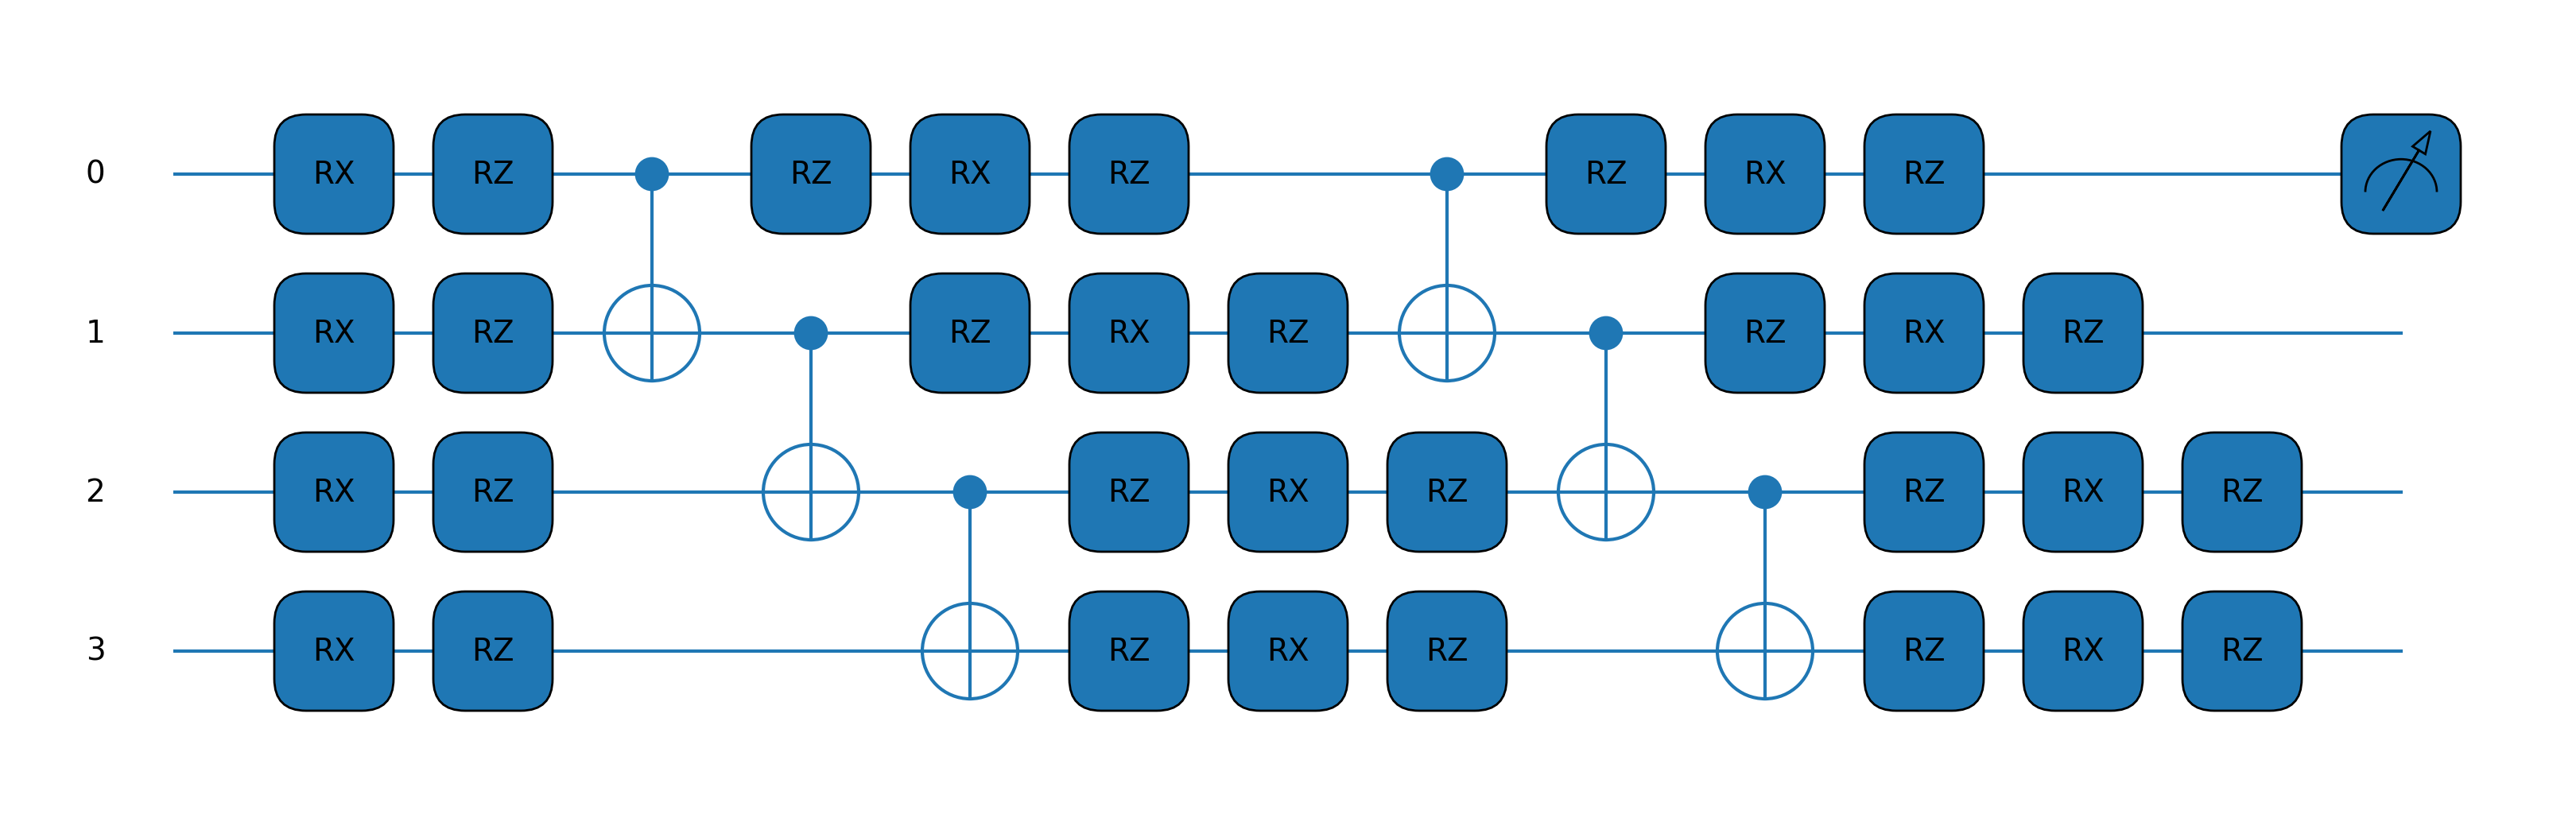
\includegraphics[width=0.47\textwidth]{a1_hea.png} & 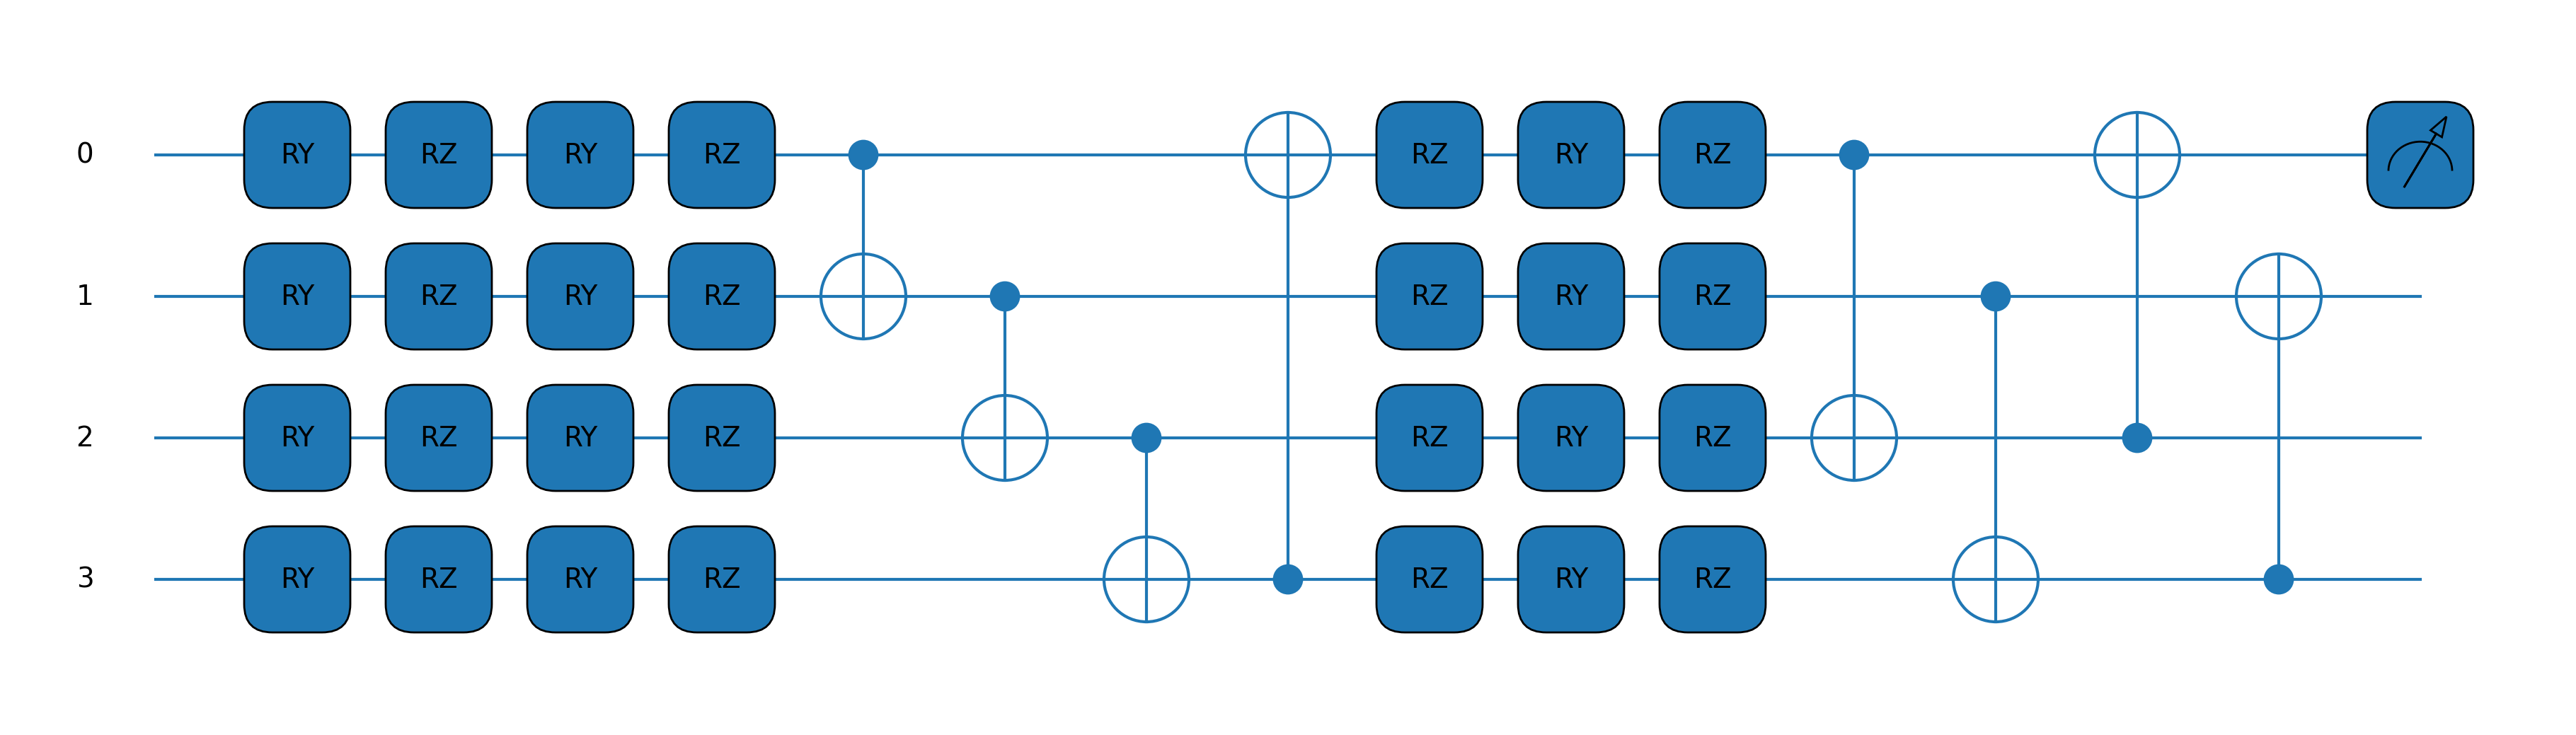
\includegraphics[width=0.47\textwidth]{a2_sel.png}\\
\scriptsize A1 HEA & \scriptsize A2 Strongly entangling\\[0.6em]
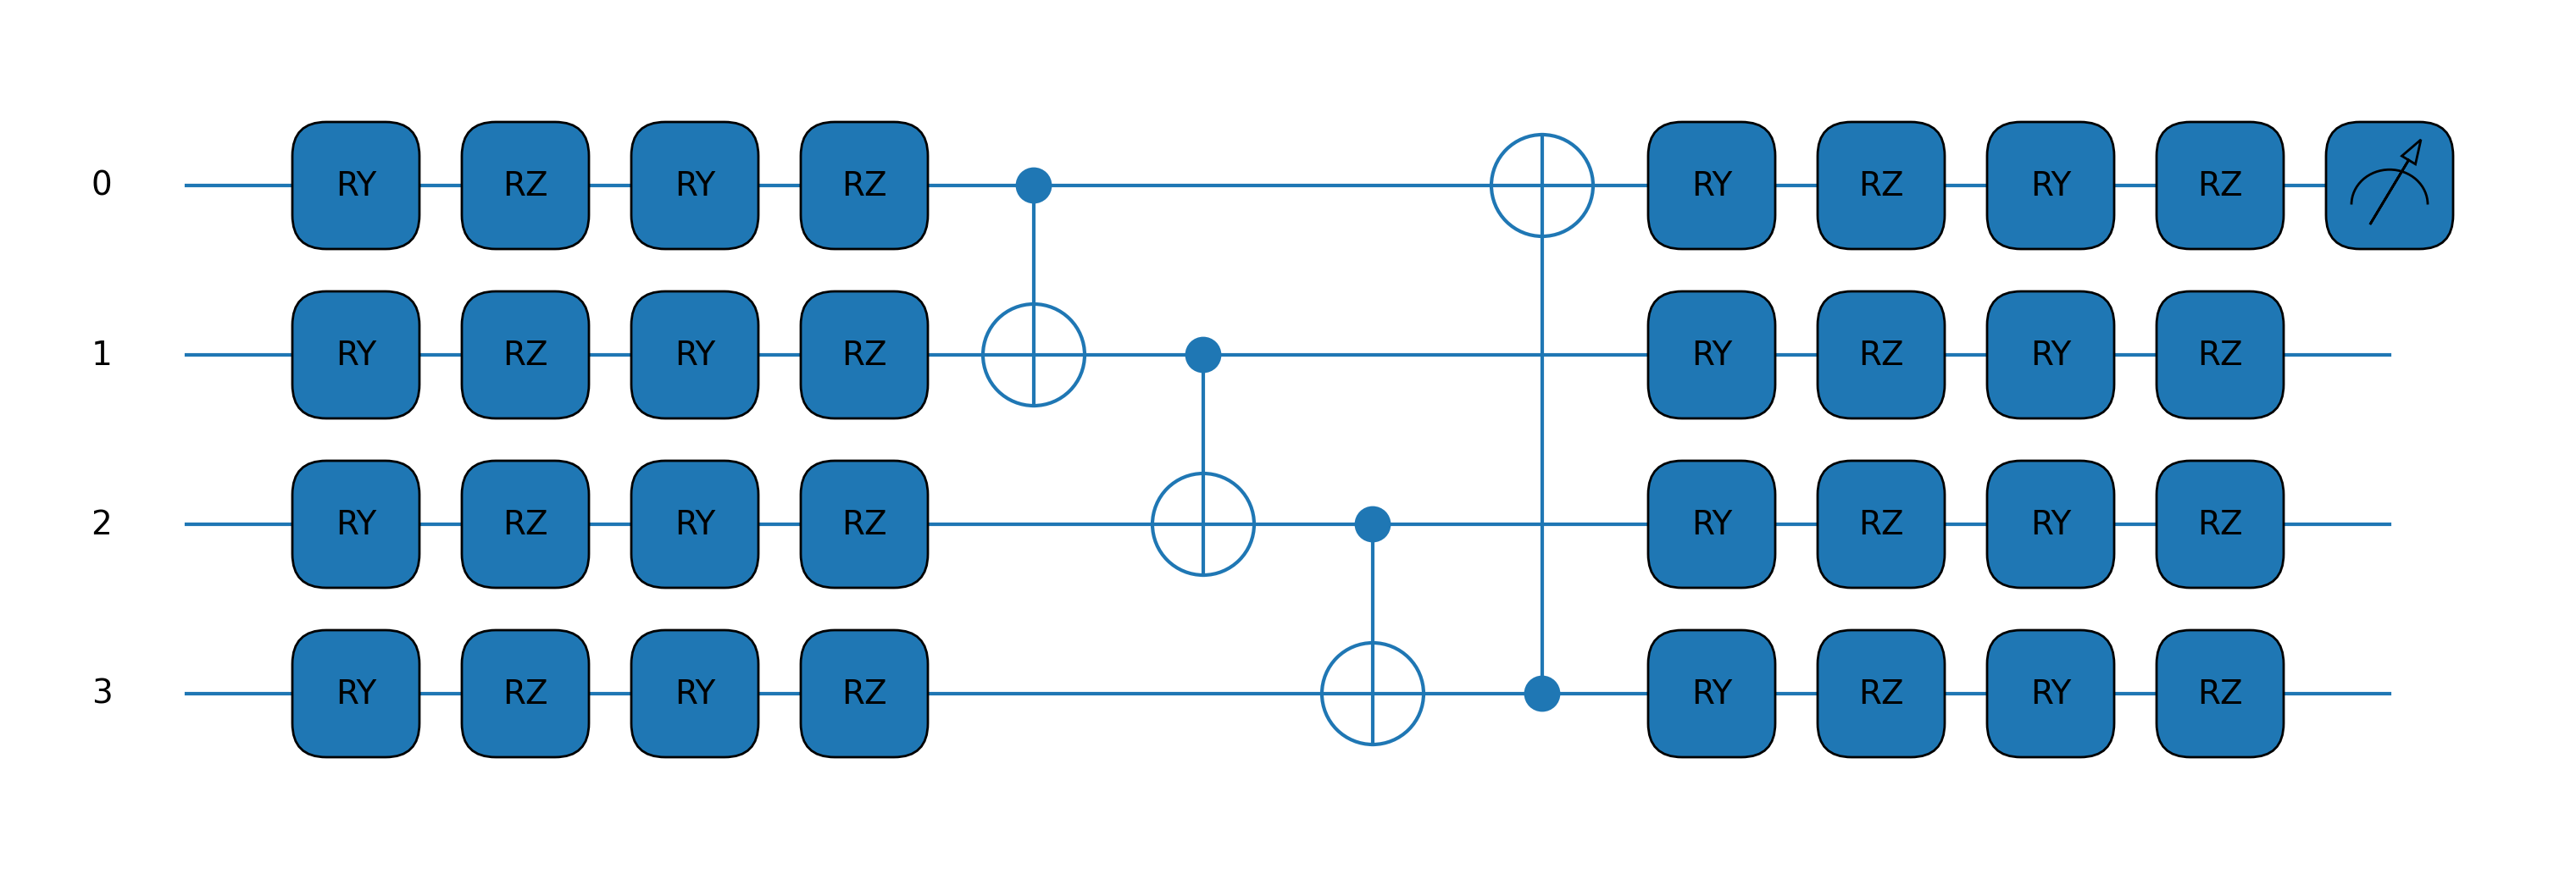
\includegraphics[width=0.47\textwidth]{a3_reupload.png} & 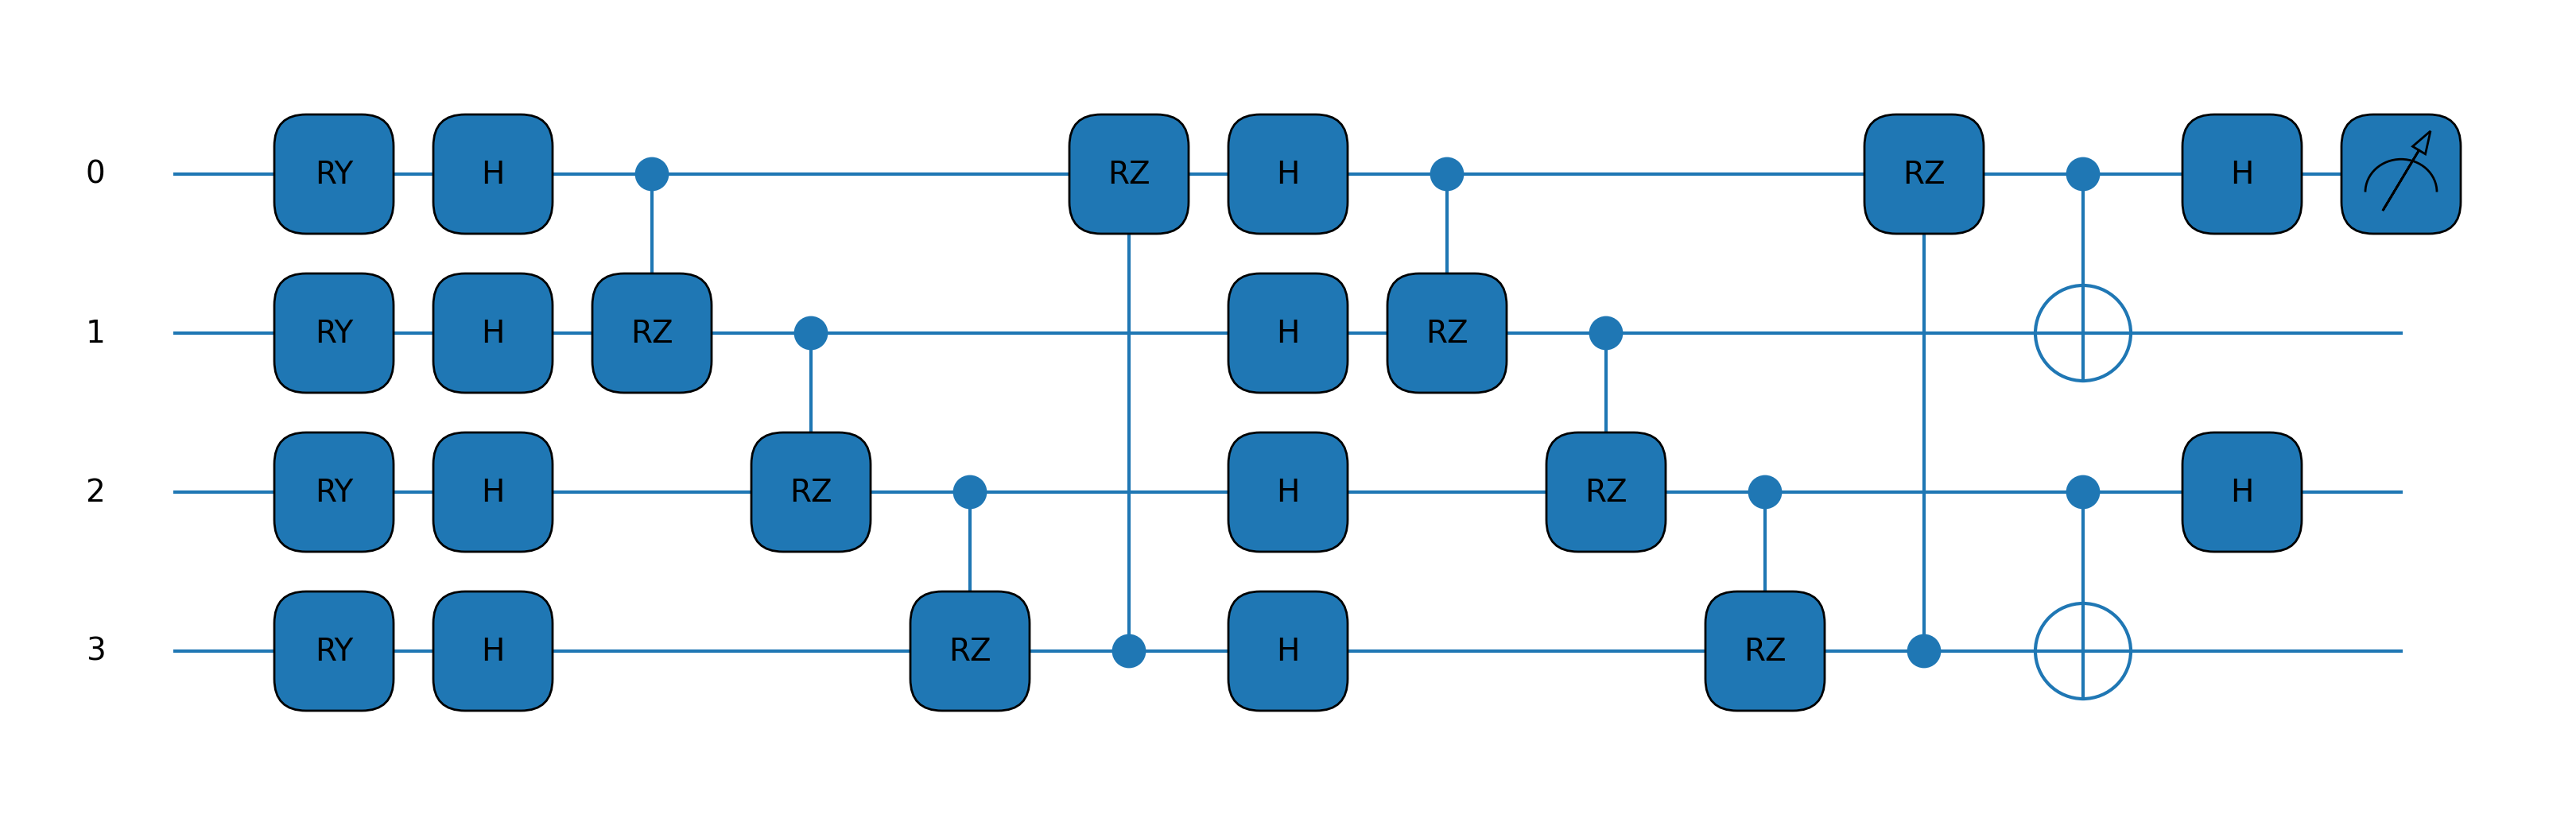
\includegraphics[width=0.47\textwidth]{a4_discocat.png}\\
\scriptsize A3 Re-uploading & \scriptsize A4 DisCoCat (plantilla)\\
\end{tabular}
\vfill
\begin{azulbox}{Lectura}
Todas las familias leen $\langle Z_0\rangle$ en el qubit 0. Los diagramas se generan desde el código (\texttt{figures/make\_diagrams.py}), no a mano.
\end{azulbox}
\end{frame}

% ---------------------------------------------------------------- 8
\begin{frame}{5. Circuitos A5 a A7}
\centering
\begin{tabular}{cc}
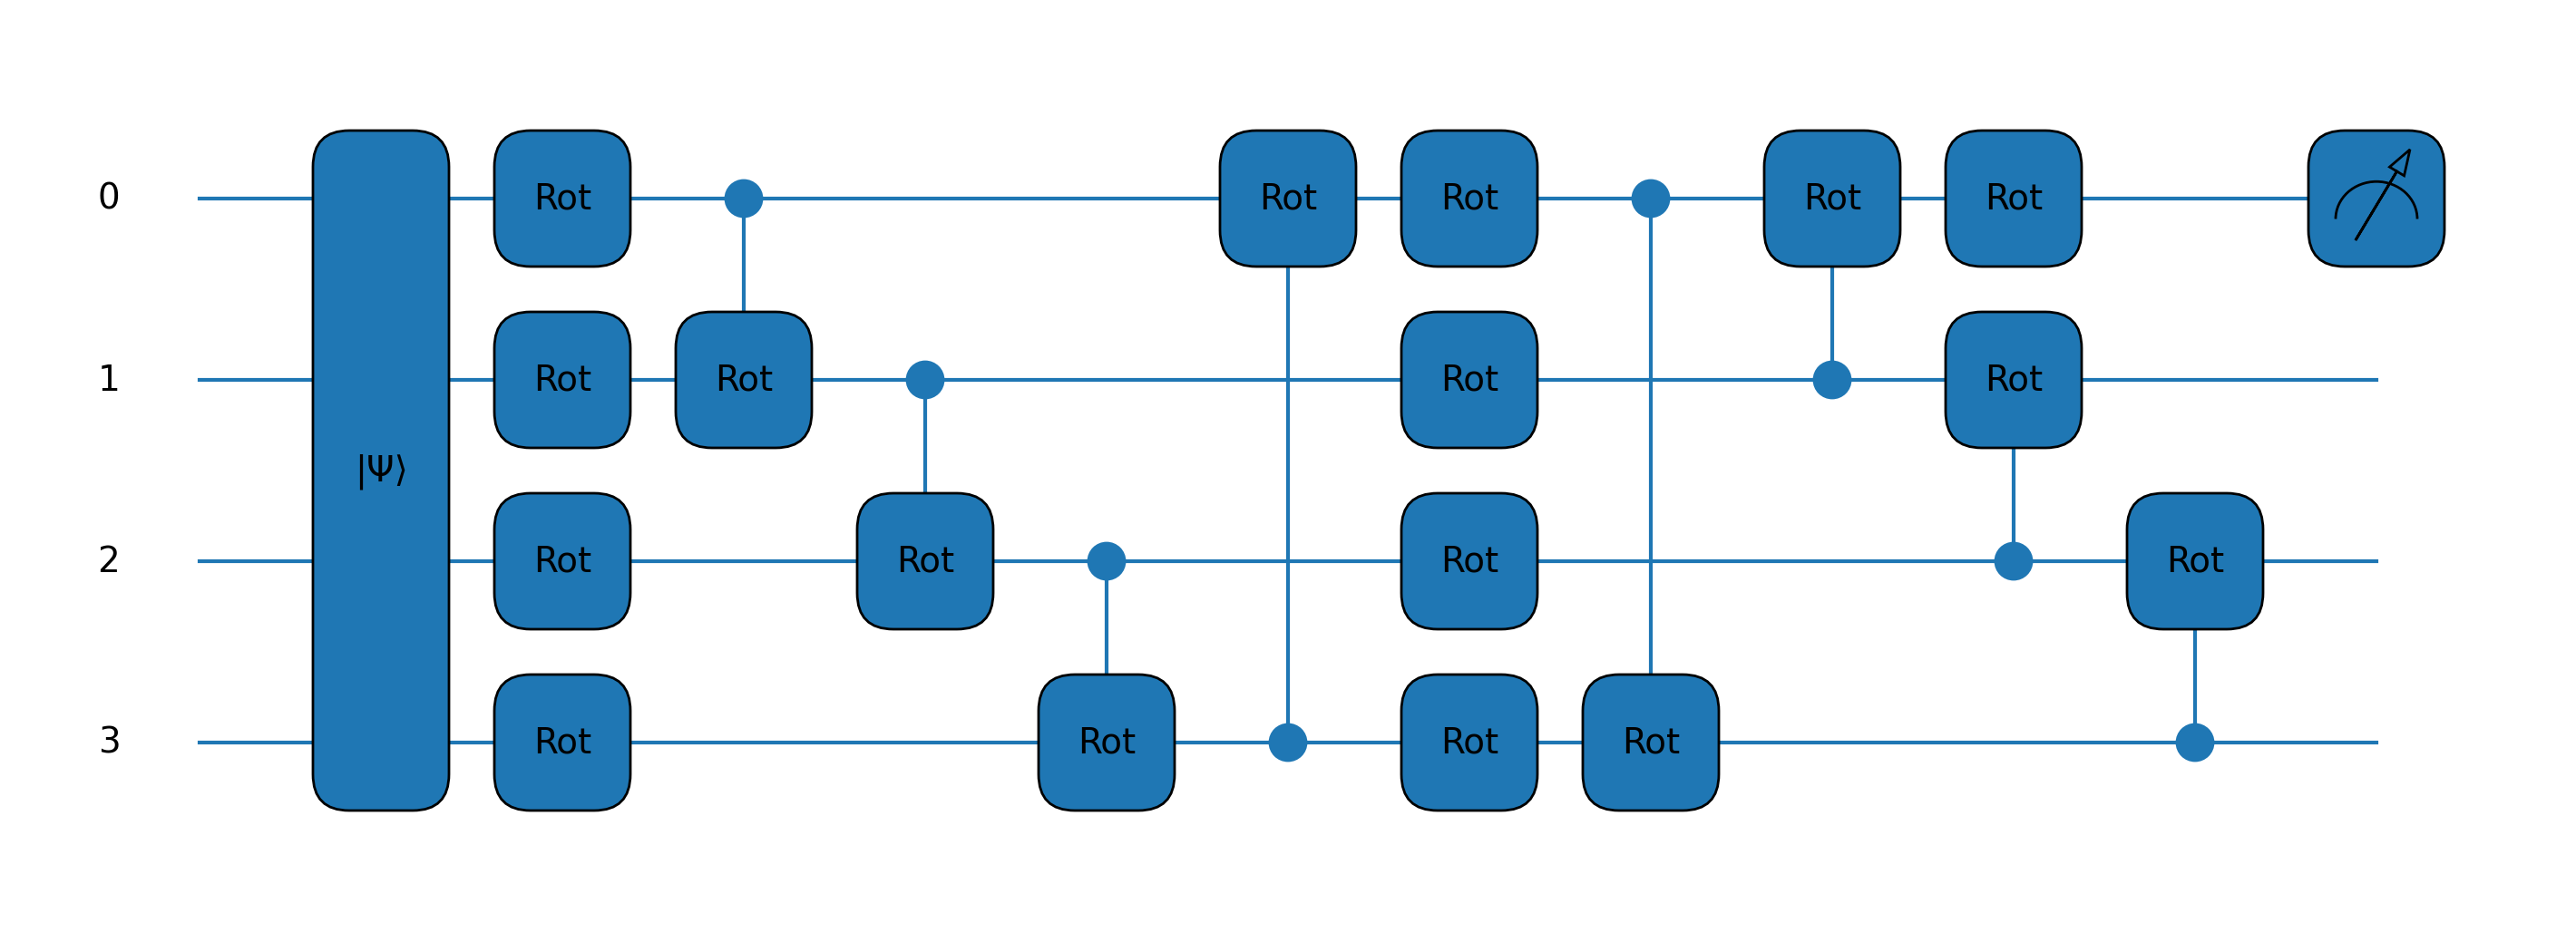
\includegraphics[width=0.47\textwidth]{a5_circuit_centric.png} & 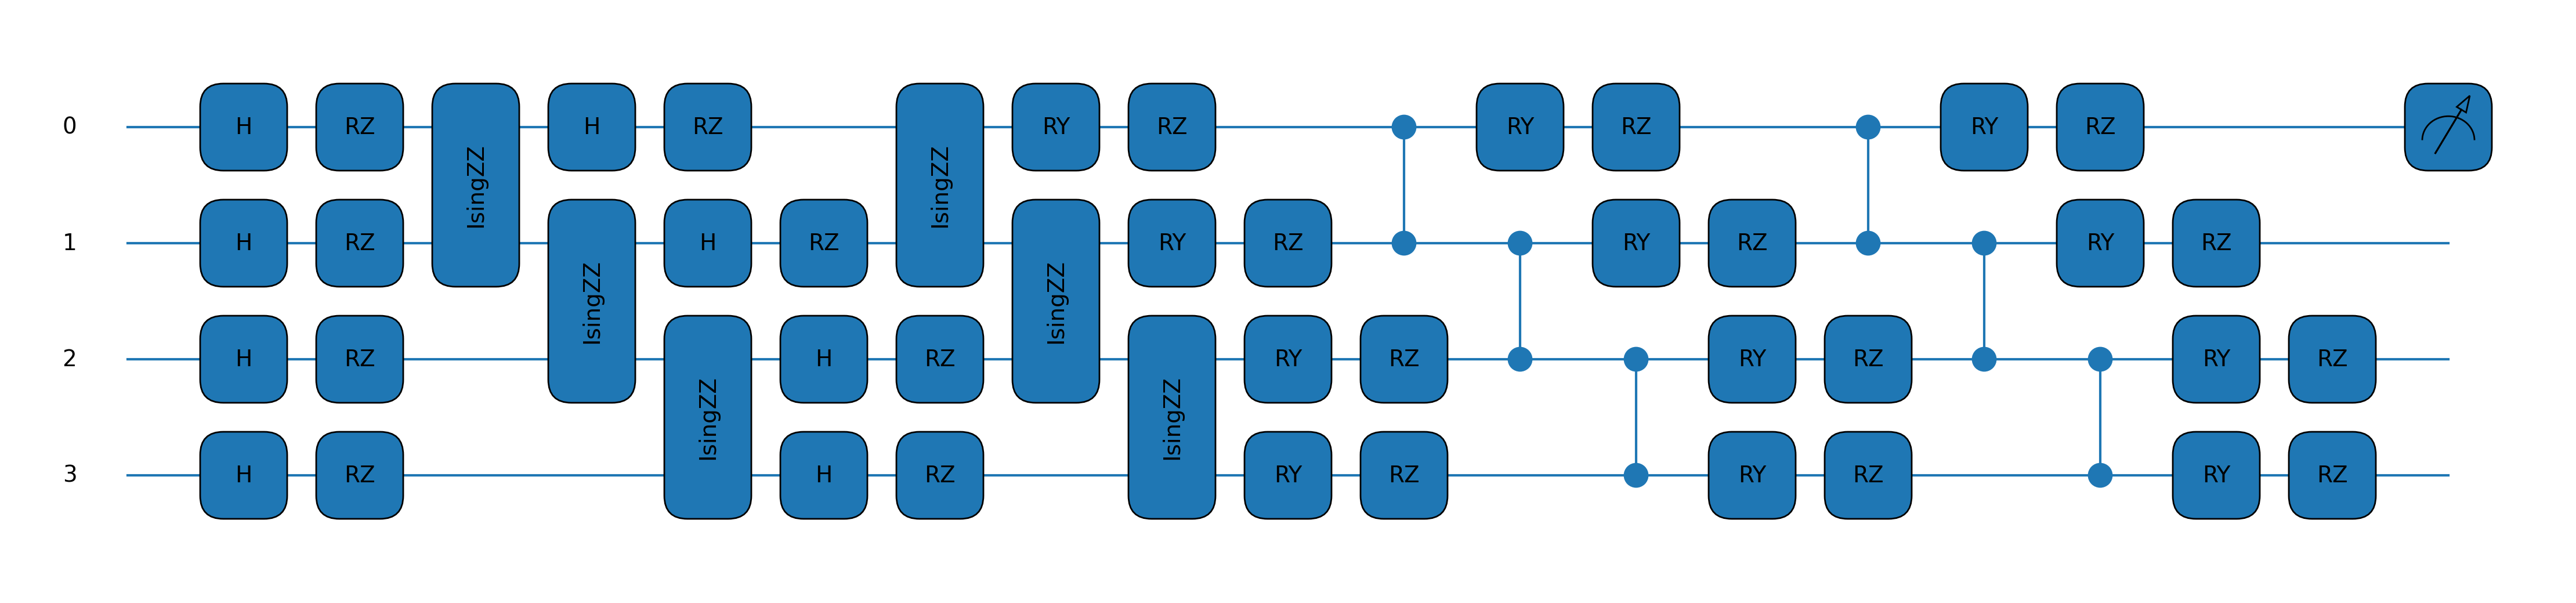
\includegraphics[width=0.47\textwidth]{a6_iqp.png}\\
\scriptsize A5 Circuit-centric & \scriptsize A6 IQP + VQC\\[0.6em]
\multicolumn{2}{c}{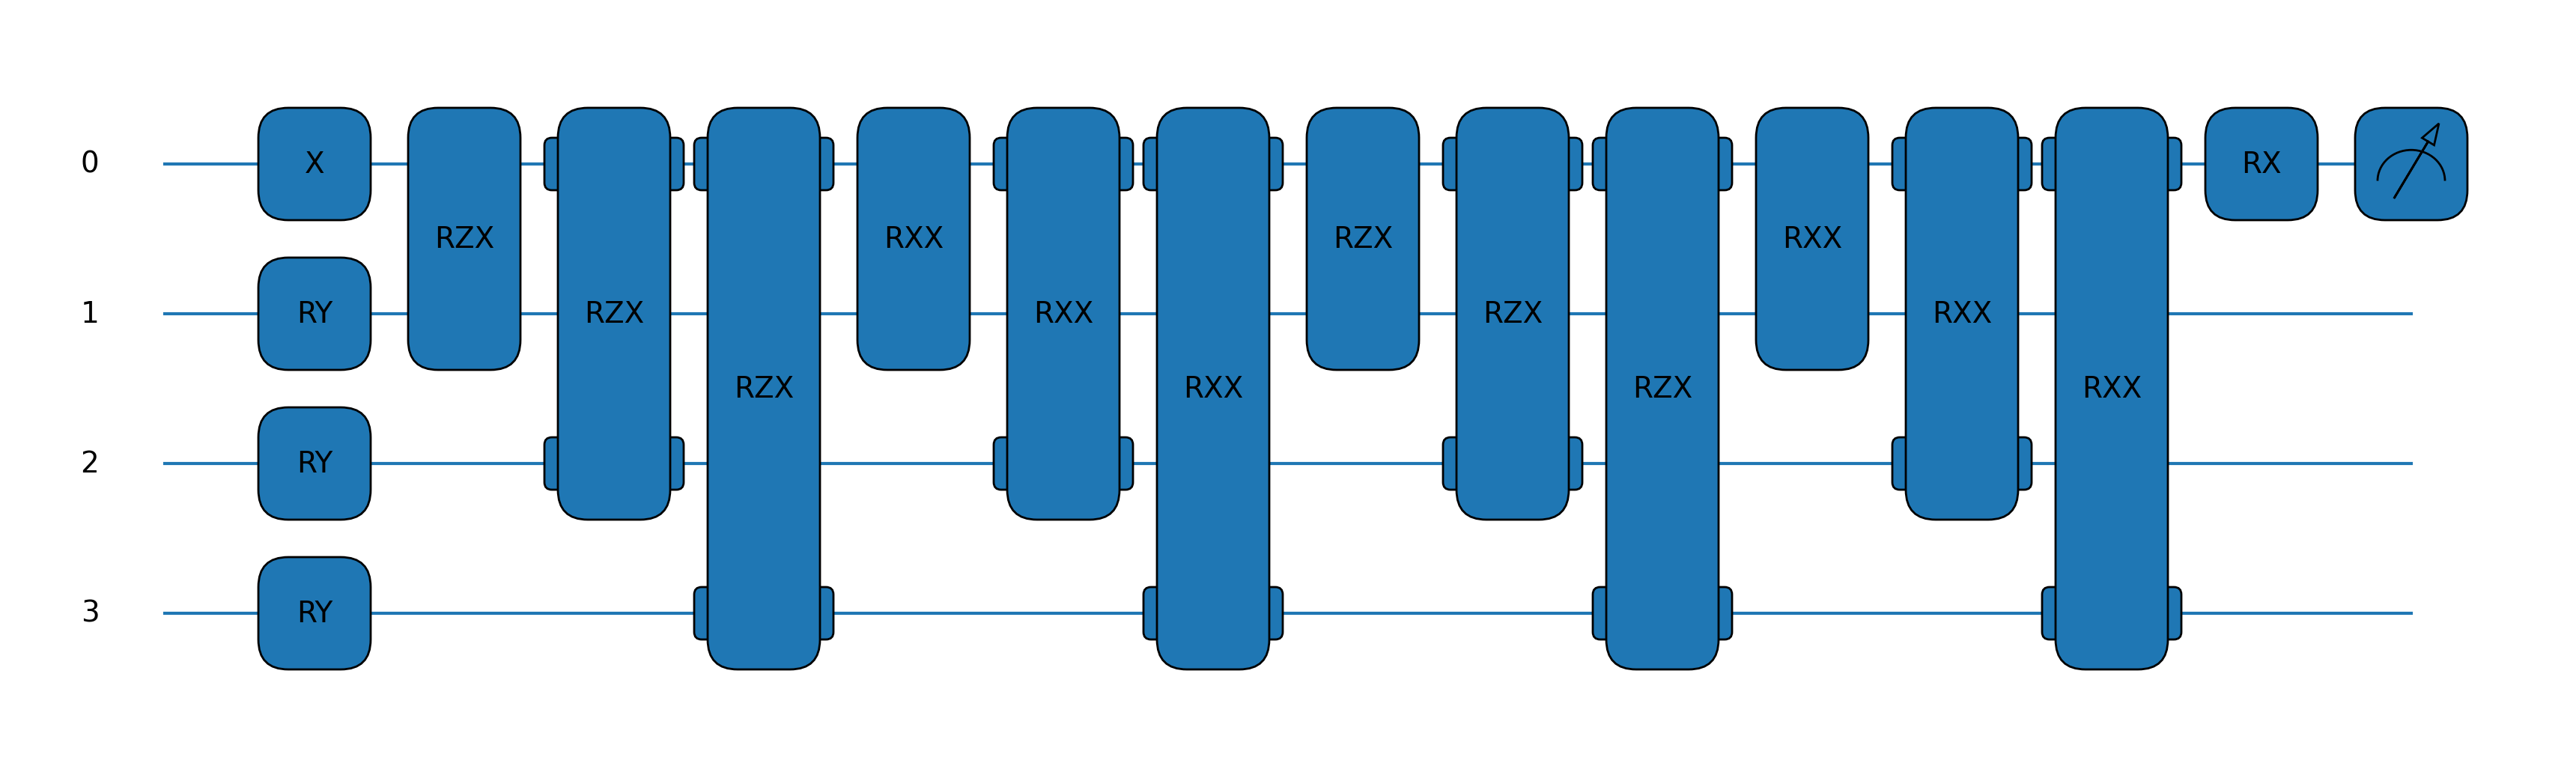
\includegraphics[width=0.47\textwidth]{a7_farhi_neven.png}}\\
\multicolumn{2}{c}{\scriptsize A7 Farhi-Neven}\\
\end{tabular}
\vfill
\begin{ambarbox}{Nota}
A7 se puede simular clásicamente en tiempo $O(nd)$: su salida es un producto de $n-1$ traslapes de un solo qubit. Se reporta junto con cualquier resultado de A7.
\end{ambarbox}
\end{frame}

% ---------------------------------------------------------------- 9
\begin{frame}{6. Descriptores del circuito: qué mide cada uno}
\small
\begin{tabularx}{\textwidth}{@{}lX@{}}
\toprule
\textbf{Tag} & \textbf{Qué mide, en palabras simples}\\
\midrule
P1 & Expresividad: qué tanto cubre el circuito el espacio de estados (distancia KL a Haar).\\
P2 & Entrelazamiento promedio que produce (Meyer-Wallach).\\
P3 & Dimensión efectiva: cuántos parámetros realmente cambian el estado.\\
P4 & Dimensión del álgebra de Lie dinámica (DLA).\\
P5, P6 & Costo: número de parámetros y de compuertas de dos qubits.\\
G1 & Varianza del gradiente al crecer $n$. Si decae como $e^{-\alpha n}$, hay \emph{barren plateau}.\\
G3 & Ancho $n^*$ donde el gradiente cae por debajo de lo que 1024 shots pueden medir.\\
G4 & Diferencia entre costo global y local.\\
G5 & Gradiente bajo ruido despolarizante.\\
G6 & Efecto de inicializar con ángulos pequeños.\\
\bottomrule
\end{tabularx}
\end{frame}

% ---------------------------------------------------------------- 10
\begin{frame}{7. Resultados: descriptores}
\small
\begin{tabularx}{\textwidth}{@{}lccccccc@{}}
\toprule
 & \textbf{A1} & \textbf{A2} & \textbf{A3} & \textbf{A4} & \textbf{A5} & \textbf{A6} & \textbf{A7}\\
\midrule
G1: $\alpha$ global ($d=5$) & 0.69 & 0.69 & 0.69 & 0.73 & 0.68 & 0.68 & 0.44\\
G3: $n^*$ (1024 shots) & 8.7 & 8.3 & 8.4 & 7.8 & 8.8 & 8.6 & no cruza\\
G6: rescate con ángulos pequeños & 1.9$\times$ & 5.6$\times$ & 0.6$\times$ & 14$\times$ & 62$\times$ & 0.3$\times$ & 35$\times$\\
\bottomrule
\end{tabularx}
\vspace{0.6em}
\begin{columns}[T]
\column{0.48\textwidth}
\begin{verdebox}{Lo que se confirma}
A1 a A6 pierden gradiente al ritmo que predice la teoría: $\alpha\approx\ln 2=0.693$. Con 1024 shots, el gradiente se vuelve inmedible cerca de 8 qubits.
\end{verdebox}
\column{0.48\textwidth}
\begin{ambarbox}{La excepción}
A7 (DLA pequeña) tiene una varianza de gradiente 22 a 38 veces mayor que A1, A2 y A4 a $n=6$, $d=5$, y no cruza el límite de shots en $n\le 10$.
\end{ambarbox}
\end{columns}
\end{frame}

% ---------------------------------------------------------------- 11
\begin{frame}{8. Resultados IMDb: mejor celda por familia (MCC en prueba)}
\small
\begin{tabularx}{\textwidth}{@{}lccccXl@{}}
\toprule
\textbf{Familia} & $n$ & $d$ & \textbf{MCC (IC 95\%)} & \textbf{Ref. logreg} & \textbf{Semillas fallidas} & \textbf{Categoría}\\
\midrule
A1 & 8 & 5 & $0.273\pm0.048$ & 0.270 & 1 de 10 & Desempeña\\
A2 & 8 & 5 & $0.262\pm0.060$ & 0.270 & 2 de 10 & Limitado por capacidad\\
A4 & 8 & 5 & $0.252\pm0.053$ & 0.270 & 3 de 10 & Limitado por entrenabilidad\\
A7 & 8 & 1 & $0.235\pm0.052$ & 0.275 & 4 de 10 & Limitado por entrenabilidad\\
A3 & 6 & 5 & $0.220\pm0.051$ & 0.283 & 4 de 10 & Limitado por entrenabilidad\\
A6 & 8 & 5 & $0.086\pm0.045$ & 0.270 & 10 de 10 & Limitado por entrenabilidad\\
A5 & 8 & 1 & $0.070\pm0.026$ & 0.424 & 10 de 10 & Limitado por entrenabilidad\\
\bottomrule
\end{tabularx}
\vspace{0.4em}
\begin{azulbox}{Cómo leer la tabla}
``Ref. logreg'' es una regresión logística con las mismas entradas que ve el circuito. ``Semilla fallida'' significa MCC menor a 0.2. Referencias fuertes: MiniLM completo 0.47, TF-IDF 0.63.
\end{azulbox}
\end{frame}

% ---------------------------------------------------------------- 12
\begin{frame}{8. Resultados IMDb: efecto del número de qubits ($d=5$)}
\small
\begin{tabularx}{\textwidth}{@{}lXXXXXXX@{}}
\toprule
$n$ & \textbf{A1} & \textbf{A2} & \textbf{A3} & \textbf{A4} & \textbf{A5} & \textbf{A6} & \textbf{A7}\\
\midrule
4 & 0.145 & 0.194 & 0.157 & 0.147 & 0.030 & 0.085 & 0.077\\
6 & 0.255 & 0.257 & 0.220 & 0.246 & 0.042 & 0.042 & 0.182\\
8 & 0.273 & 0.262 & 0.220 & 0.252 & $-$0.009 & 0.087 & 0.159\\
\bottomrule
\end{tabularx}
\vspace{0.6em}
\begin{columns}[T]
\column{0.48\textwidth}
\begin{verdebox}{Patrón}
Las familias de ángulo (A1 a A4) mejoran de 4 a 6 qubits y luego se aplanan. Siguen de cerca a la regresión logística con las mismas features: el límite lo pone la información que entra, no el circuito.
\end{verdebox}
\column{0.48\textwidth}
\begin{ambarbox}{Las que no aprenden}
A5 (amplitud) y A6 (IQP) quedan cerca de cero en todas las celdas, aunque A5 recibe más información (PCA de $2^n$ componentes).
\end{ambarbox}
\end{columns}
\end{frame}

% ---------------------------------------------------------------- 13
\begin{frame}{8. Resultados: categorías y CoLA}
\begin{columns}[T]
\column{0.48\textwidth}
\small
\textbf{IMDb, 69 celdas}\\[0.3em]
\begin{tabular}{@{}lr@{}}
\toprule
Categoría & Celdas\\
\midrule
Limitado por entrenabilidad & 46\\
Piso (MCC no distinto de 0) & 16\\
Limitado por capacidad & 6\\
Desempeña & 1\\
\bottomrule
\end{tabular}
\vspace{0.5em}
\begin{azulbox}{Lectura}
El problema dominante es entrenar: con inicialización uniforme muchas semillas no despegan, sobre todo a $d=1$.
\end{azulbox}
\column{0.48\textwidth}
\begin{ambarbox}{CoLA (aceptabilidad gramatical)}
A $n=4$, las 27 celdas quedan en el piso: MCC entre $-0.03$ y $+0.03$. La regresión logística con las mismas features también da 0.00. El problema está en la representación (MiniLM + PCA a 4 componentes no conserva la señal sintáctica), antes del circuito.
\end{ambarbox}
\begin{ambarbox}{Pendiente}
CoLA a $n=6$ y $n=8$: 42 celdas sin correr.
\end{ambarbox}
\end{columns}
\end{frame}

% ---------------------------------------------------------------- 14
\begin{frame}{9. Resultados: ruido de hardware ($n=4$, IMDb)}
\begin{azulbox}{Qué se hizo}
Modelos entrenados sin ruido se evaluaron con ruido despolarizante, bit flip y phase flip, con tasa de dos qubits 10 veces la de un qubit. Nivel NISQ: $10^{-3}$ y $10^{-2}$.
\end{azulbox}
\begin{columns}[T]
\column{0.48\textwidth}
\begin{verdebox}{Resultado}
En las 21 celdas, la pérdida de MCC está entre $-0.011$ y $+0.020$, debajo del SESOI de 0.03. A $n=4$ ninguna familia queda limitada por ruido.
\end{verdebox}
\column{0.48\textwidth}
\begin{ambarbox}{Qué predice la pérdida}
El número de compuertas de dos qubits predice la pérdida mejor que la profundidad ($\rho=0.81$ contra $0.68$). Esto contradice la hipótesis H7.
\end{ambarbox}
\end{columns}
\end{frame}

% ---------------------------------------------------------------- 15
\begin{frame}{10. Hipótesis pre-registradas: veredictos}
\scriptsize
\begin{tabularx}{\textwidth}{@{}lXl@{}}
\toprule
\textbf{ID} & \textbf{Predicción (simplificada) y lo que pasó} & \textbf{Veredicto}\\
\midrule
H1 & El gradiente decae con $n$ y el costo local decae mucho más lento. Se cumple en A1, A4, A5, A6; falla en A2, A3 y A7. & Refutada\\
H2 & A $n=6$ el gradiente cae con la profundidad y se estabiliza. Ninguna familia cae con $d$. & Refutada\\
H3 & $d=3$ mejora a $d=1$, y $d=5$ no agrega más. Solo A3 (y A4 a $n=8$) mejora con significancia; el resto queda inconcluso. & Refutada\\
H4 & $n=6$ mejora a $n=4$, y $n=8$ no agrega más. Solo A7 mejora con significancia ($d=1$ y $d=3$). & Refutada\\
H5 & (a) A1, A2, A4, A7 equivalentes: no se demuestra. (b) A7 con más gradiente: sí. (c) A1 a $d=1$ con más fallas: sí. & Refutada (a)\\
H6 & Re-upload y amplitud superan a ángulo; IQP no supera a ángulo. Amplitud queda peor; IQP se cumple. & Refutada\\
H7 & La profundidad predice la pérdida por ruido mejor que las compuertas de dos qubits. Fue al revés. & Refutada\\
H8 & El orden entre familias es más consistente que en fair-v1. Falta el cálculo de fair-v1. & Incompleta\\
\bottomrule
\end{tabularx}
\vspace{0.3em}
\begin{azulbox}{Por qué tantas refutadas}
Una hipótesis se marca refutada si cualquier parte falla. Muchas partes salen inconclusas con 10 semillas. Un resultado refutado también es un resultado: se reporta tal como se escribió antes de los datos.
\end{azulbox}
\end{frame}

% ---------------------------------------------------------------- 16
\begin{frame}{10. Limitaciones declaradas}
\small
\begin{columns}[T]
\column{0.48\textwidth}
\begin{ambarbox}{Diferencias con los artículos}
A4 no post-selecciona las ``cups'' y no usa un parser. A5 a $n=6$ tiene más compuertas controladas que la regla del artículo. A6 recibe ángulos en $[0,\pi]$, no en $(0,2\pi]$. Todo está declarado en \texttt{docs/IMPLEMENTATION.md} y probado en \texttt{tests/test\_conventions.py}.
\end{ambarbox}
\column{0.48\textwidth}
\begin{ambarbox}{Límites del diseño}
El contraste A3 contra A2 cambia la codificación y el entrelazador a la vez. La inicialización uniforme favorece las fallas; G6 muestra que ángulos pequeños ayudarían a A4, A5 y A7. Todo es simulación exacta, no hardware.
\end{ambarbox}
\end{columns}
\end{frame}

% ---------------------------------------------------------------- 17
\begin{frame}[fragile]{11. Repositorio y reproducibilidad}
\begin{columns}[T]
\column{0.44\textwidth}
\scriptsize
\begin{verbatim}
vqc_scorecard/
  ansatze/   A1 a A7, un archivo cada una
  probes/    física: gradientes, DLA, QFIM
  metrics/   P1 a P6, G1 a G6
  tasks/     datos, modelo, protocolo
  noise/     modelos de ruido
  tests/     239 pruebas
  results/   JSON y JSONL de todo
  docs/      implementación, pre-registro
\end{verbatim}
\column{0.54\textwidth}
\begin{azulbox}{Reproducir}
\scriptsize\texttt{pip install -r requirements.txt}\\
\texttt{python -m vqc\_scorecard.tests}\\
\texttt{python -m vqc\_scorecard.tasks.pure\_report}\\
\texttt{python -m vqc\_scorecard.figures.export\_pure\_tables}
\end{azulbox}
\begin{verdebox}{Garantías}
Versiones fijas (PennyLane 0.42.3, NumPy 2.4.4). Cada resultado lleva el digest del protocolo (\texttt{b2833a59e87d}). Las tablas de esta presentación salen de \texttt{results/pure/cells.csv}.
\end{verdebox}
\end{columns}
\end{frame}

% ---------------------------------------------------------------- 18
\begin{frame}{12. Pendientes para cerrar}
\small
\begin{tabularx}{\textwidth}{@{}Xll@{}}
\toprule
\textbf{Tarea} & \textbf{Qué falta} & \textbf{Estado}\\
\midrule
CoLA a $n=6$ y $n=8$ & 42 celdas de 10 semillas & \pend\\
H8 & Coeficiente $W$ de Kendall de fair-v1 a $n=4$, $d=3$ & \pend\\
G5 para A5 a A7 & Barrido de ruido en descriptores & \pend\\
Publicación del repositorio & GitHub, etiqueta de versión, DOI (Zenodo) & \pend\\
\bottomrule
\end{tabularx}
\end{frame}

% ---------------------------------------------------------------- 19
\begin{frame}{12. Conclusiones}
\begin{itemize}\setlength{\itemsep}{0.5em}
\item Seis de siete familias pierden gradiente al ritmo que predice la teoría ($\alpha\approx\ln 2$). La única excepción, A7, tiene una DLA pequeña y es simulable clásicamente.
\item Cuando solo el circuito aprende, las familias de ángulo (A1 a A4) llegan al nivel de una regresión logística con las mismas features, y no lo superan.
\item Amplitud (A5) e IQP (A6) no aprenden la tarea en este protocolo.
\item El cuello de botella principal es entrenar, no el ruido: a $n=4$ el ruido NISQ cambia el MCC menos de 0.03.
\item En CoLA, la representación de entrada no tiene la señal; ningún circuito la puede recuperar.
\end{itemize}
\end{frame}

% ---------------------------------------------------------------- 20
\begin{frame}{Referencias}
\scriptsize
\begin{itemize}
\item Kandala, A. et al. (2017). Hardware-efficient variational quantum eigensolver for small molecules and quantum magnets. \emph{Nature}, 549, 242.
\item Schuld, M., Bocharov, A., Svore, K. M., Wiebe, N. (2020). Circuit-centric quantum classifiers. \emph{Phys. Rev. A}, 101, 032308.
\item Pérez-Salinas, A., Cervera-Lierta, A., Gil-Fuster, E., Latorre, J. I. (2020). Data re-uploading for a universal quantum classifier. \emph{Quantum}, 4, 226.
\item Meichanetzidis, K., Gogioso, S., de Felice, G., Chiappori, N., Toumi, A., Coecke, B. (2020). Quantum natural language processing on near-term quantum computers. arXiv:2005.04147.
\item Havlíček, V. et al. (2019). Supervised learning with quantum-enhanced feature spaces. \emph{Nature}, 567, 209.
\item Farhi, E., Neven, H. (2018). Classification with quantum neural networks on near term processors. arXiv:1802.06002.
\item Ragone, M. et al. (2024). A Lie algebraic theory of barren plateaus for deep parameterized quantum circuits. \emph{Nature Communications}, 15, 7172.
\item Larocca, M. et al. (2025). Barren plateaus in variational quantum computing. \emph{Nature Reviews Physics}, 7, 174.
\end{itemize}
\end{frame}

\end{document}
